% This is a simple sample document.  For more complicated documents take a look in the exercise tab. Note that everything that comes after a % symbol is treated as comment and ignored when the code is compiled.

\documentclass{article} % \documentclass{} is the first command in any LaTeX code.  It is used to define what kind of document you are creating such as an article or a book, and begins the document preamble

\usepackage{amsmath} % \usepackage is a command that allows you to add functionality to your LaTeX code
\usepackage{tikz} % This package allows you to create graphs and diagrams

\title{Simple Sample} % Sets article title
\author{My Name} % Sets authors name
\date{\today} % Sets date for date compiled

% The preamble ends with the command \begin{document}
\begin{document} % All begin commands must be paired with an end command somewhere
\maketitle % creates title using information in preamble (title, author, date)

\section{Hello World!} % creates a section

\textbf{Hello World!} Today I am learning \LaTeX. %notice how the command will end at the first non-alphabet charecter such as the . after \LaTeX
\LaTeX{} is a great program for writing math. I can write in line math such as $a^2+b^2=c^2$ %$ tells LaTexX to compile as math
. I can also give equations their own space:
\begin{equation} % Creates an equation environment and is compiled as math
  \gamma^2+\theta^2=\omega^2
\end{equation}
If I do not leave any blank lines \LaTeX{} will continue  this text without making it into a new paragraph.  Notice how there was no indentation in the text after equation (1).
Also notice how even though I hit enter after that sentence and here $\downarrow$
\LaTeX{} formats the sentence without any break.  Also   look  how      it   doesn't     matter          how    many  spaces     I put     between       my    words.

For a new essay I can leave a blank space in my code.

is this ok ?

Yes it is!

But can it also create new paragraphs?

Yes!  By leaving a blank line in the code I can create a new paragraph.

So let's try it again.

We now want to create a graph. I want a graph with 5 vertices, all connected to each other.  This is called a complete graph on 5 vertices, or $K_5$.
Below is the code to create this graph using the tikz package.

This is another change:


\begin{center} % centers the figure
  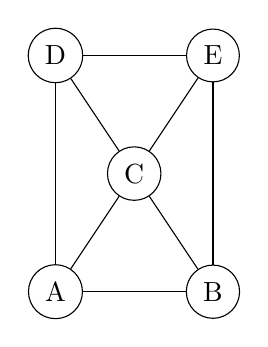
\begin{tikzpicture} % begins the tikz environment
    \node (A) at (0,0) [circle,draw] {A
    };
    \node (B) at (2,0) [circle,draw] {B
    };
    \node (C) at (1,1.5) [circle,draw] {C
    };
    \node (D) at (0,3) [circle,draw] {D
    };
    \node (E) at (2,3) [circle,draw] {E
    };
    \draw (A) -- (C);
    \draw (A) -- (D);
    \draw (A) -- (B);
    \draw (B) -- (C);
    \draw (B) -- (E);
    \draw (C) -- (D);
    \draw (C) -- (E);
    \draw (D) -- (E);
  \end{tikzpicture}
\end{center} % ends centering


\section{Lists} % creates another section
I can also make lists:
\begin{itemize} % creates an itemized list
  \item First Item
  \item Second Item
  \item Third Item
  \item  Fourth Item
\end{itemize}

\end{document} % This is the end of the document